\section*{Assignment 08: Metrics and Learning}
\addcontentsline{toc}{section}{Assignment 08: Metrics and Learning}

Here I focus on the metrics that actually matter for SkillSync so the platform feels good in practice and performs on paper. The English write-up stays grounded so we can use it day to day rather than as an academic artefact.

\subsection*{KPIs that make sense}
\begin{itemize}
    \item \textbf{Matching rate}: Share of suggested matches that land. If it drops we tweak the algorithm or onboarding questions and slice by cohort to see whether campaigns or new verticals drag the average.
    \item \textbf{Repeat usage rate}: Share of users who return within 30 days. A dip triggers a review of retention features, notifications, or community events.
    \item \textbf{Net Promoter Score}: Still useful because it shows whether people would recommend us. A dip often flags fairness or bugs, so we pair it with quick interviews.
    \item \textbf{Time-to-first-value}: Minutes to the first meaningful interaction. If it drags, we strip friction or add guided missions.
    \item \textbf{Revenue per active match}: Keeps monetisation tied to behaviour. We also watch variance so a few power users do not prop up the number.
    \item \textbf{Equity of participation}: Share of projects coming from resource-light partners so we stay honest about the inclusion goals from Assignment~07.
\end{itemize}

\subsection*{Data infrastructure and feedback loop}
I keep the data stack simple. Events land in a cloud warehouse (BigQuery or Snowflake), we stream via Segment or RudderStack so the app stays decoupled, dbt shapes clean tables for analysis, and dashboards live in a shared Looker Studio or Metabase space so anyone can explore without SQL.

The feedback loop runs on three rhythms, mirroring the instrumentation drills from Lecture~5 on metrics and experimentation \citep{Lecture05}:
\begin{itemize}
    \item \textbf{Weekly reviews}: Product, data, and support meet every Tuesday, walk the KPI dashboard, and check fresh cohorts so onboarding issues surface fast.
    \item \textbf{Monthly cohort analyses}: Segment by acquisition channel and first-match timestamp to see which cohorts stick and pay; the report feeds marketing spend and the roadmap.
    \item \textbf{Quarterly learning readouts}: Summarise experiments, share surprises, and reset hypotheses so the informal student vibe still produces structured knowledge.
\end{itemize}

\subsection*{How metrics guide change}
Imagine matching rate drops from 62\% to 48\% over three weeks. Weekly review shows it is new users from a partner campaign and the cohort analysis reveals time-to-first-value above 48 hours. We run an onboarding A/B test, add a preference step, tighten algorithm weights, and ship the winner two sprints later. The next monthly check shows matching above 60\%, repeat usage up eight points, revenue per active match nudging upward, and equity of participation still intact, turning KPIs into a compass instead of decoration.

Figure~\ref{fig:feedback-screen} shows the feedback interface powering these metrics. After each project both sides rate collaboration quality, delivery against scope, and communication cadence; qualitative notes surface for moderation while scores flow into the matching algorithm. ``Impact badges'' reinforce good behaviour and the updated `Student-Project-Feedback.png` proves the UX stays light while data stays rich.

\begin{figure}[h]
  \centering
  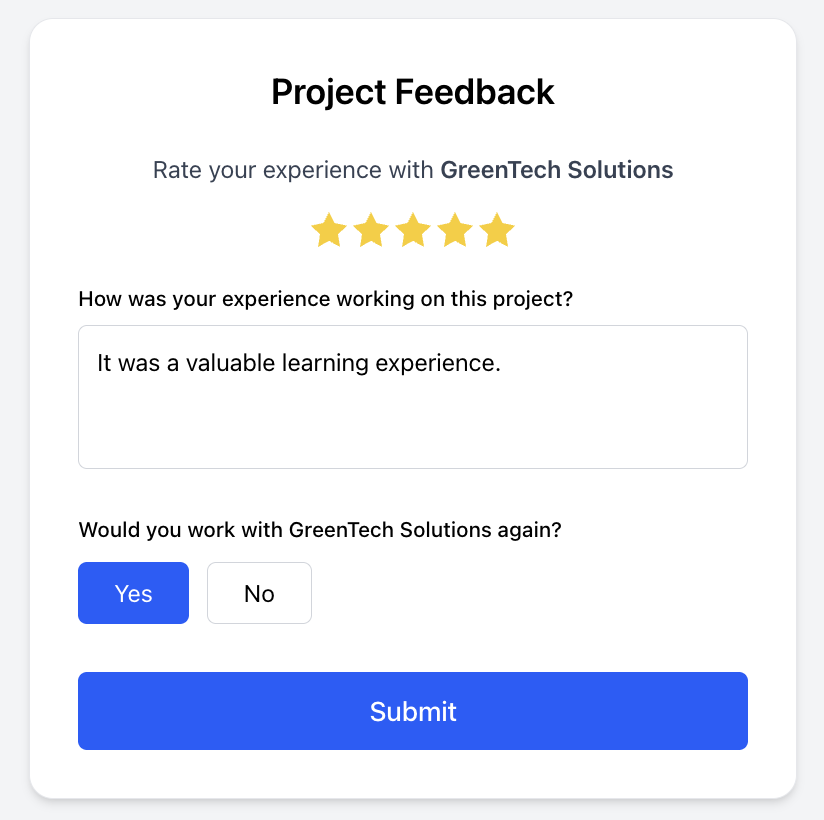
\includegraphics[width=0.8\linewidth]{figures/Student-Project-Feedback.png}
  \caption{Feedback and evaluation screen (`Student-Project-Feedback.png`) that powers the KPI loop.}
  \label{fig:feedback-screen}
\end{figure}

We built the analytics stack for reproducibility. Dashboards carry ``definition'' tooltips that link to the dbt logic, SQL lives in version control, and a metrics catalogue keeps newcomers oriented. Quarterly KPI snapshots preserve history even as definitions evolve, turning metrics into institutional memory in the spirit of \citet{Choudary2016}.
